% ! TeX root = ../../master-thesis.tex

\section{Simulator}
\label{section:implementation:simulator}

The implementation of a simulator is depicted by the class diagram in Figure
\ref{figure:simulator-class-diagram}, which is based on the design described in
Section \ref{section:design:simulation}.

\begin{figure}[!ht]
  \centering
  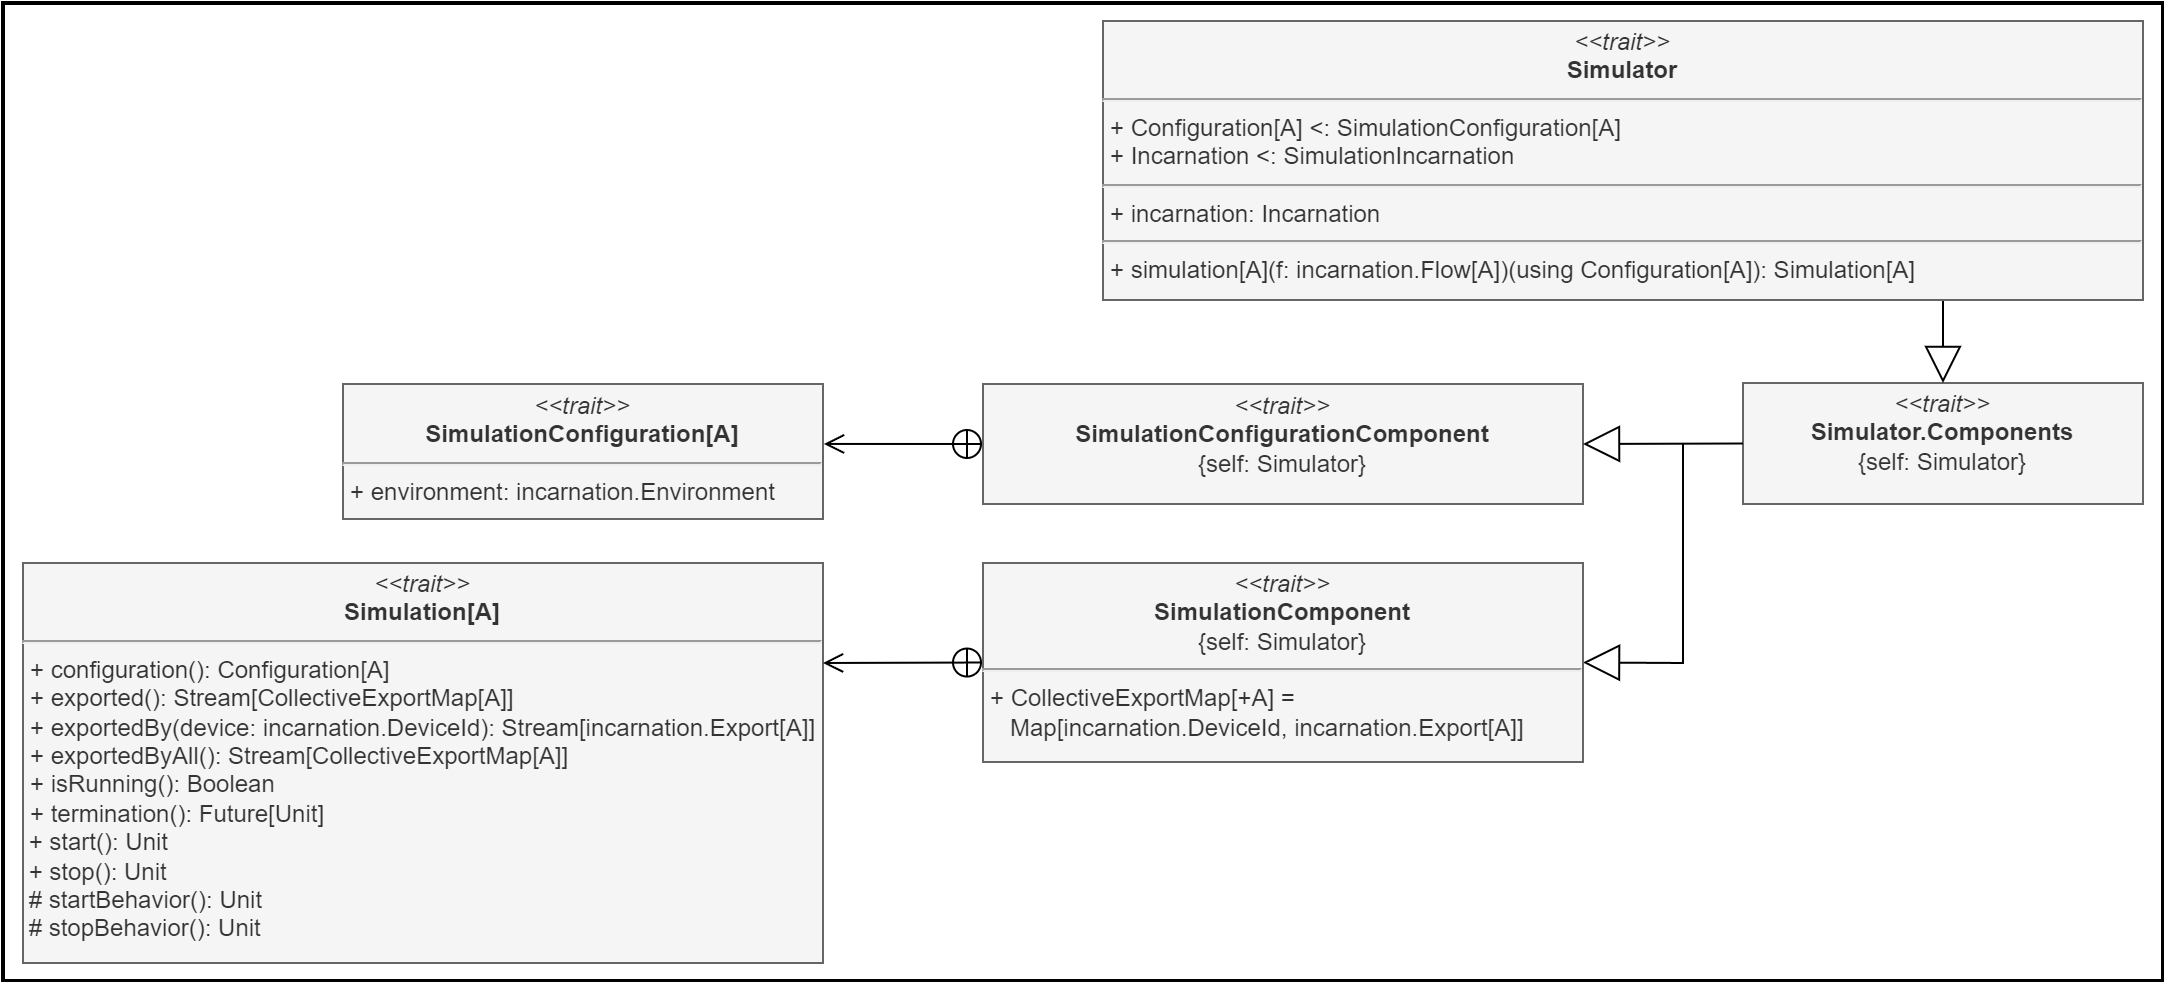
\includegraphics[width=1\textwidth]{resources/figures/simulator-class-diagram.png}
  \caption[A UML class diagram of the simulator]{
    A UML class diagram of the simulator and its components.
  }
  \label{figure:simulator-class-diagram}
\end{figure}

A \texttt{Simulator} can be used to create several \texttt{Simulation}s, each
one requiring a \texttt{Flow}, that is a FRASP specification, and a
\texttt{Configuration}, which includes the \texttt{Environment} where the
aggregate is situated. To define the concepts of \texttt{Flow} and
\texttt{Environment}, a \texttt{Simulator} relies on a specific
\texttt{SimulationIncarnation}, which is an instance of the aggregate computing
\ac{DSL} in FRASP, tailored for simulation.

The implementation of the \texttt{Simulator} follows the \textit{cake pattern},
in which dependencies are defined inside external mixin components and can be
imported by extending the desired components. In particular, \texttt{Simulator}
depends on the \texttt{Simula\-tionConfigurationComponent}, which defines the
concept of \texttt{SimulationConfi\-guration}, and the
\texttt{SimulationCompo\-nent}, which defines the concept of
\texttt{Simula\-tion}. In the following sections, specializations of
\texttt{Simulator} defines additional concepts using other components, adhering
to the same naming convention.

As per design, a \texttt{Simulation} provides observability by means of the
methods \texttt{exported}, which supplies a \texttt{Stream} of all the device
exports transmitted within the aggregate, \texttt{exportedBy}, which supplies a
\texttt{Stream} of all the exports of a single device (\textit{an individual
view}), and \texttt{exportedByAll}, which supplies a \texttt{Stream} of all the
device exports accumulated during the simulation (\textit{a global view}, in
which each event is a \texttt{CollectiveExportMap}, that is a map from the
devices to their latest export). Similar methods are provided to observe only
the result of the computations, that is the root of the device exports.

Concerning controllability, a \texttt{Simulation} exposes one method
\texttt{start} to begin its execution, running the underlying
\texttt{startBehavior} of the concrete type of \texttt{Simulation}, and another
method \texttt{stop} to halt it, running the underlying \texttt{stopBehavior}
likewise. Moreover, a method \texttt{isRunning} can be used to know if the
simulation has already started but has not stopped yet, while another method
\texttt{termination} allows reacting to the end of the simulation.
